\documentclass[10pt]{beamer}

%%%
% PREAMBLE FOR THIS DOC 
%%%
%https://tex.stackexchange.com/questions/68821/is-it-possible-to-create-a-latex-preamble-header
\usepackage{/Users/miw267/Repos/csci246_spring2025/slides/preambles/beamer_preamble_for_CSCI246}

\usetikzlibrary{matrix}

\usetikzlibrary{shapes.geometric}

\usepackage{pgfplots} % For drawing histograms
\usetikzlibrary{pgfplots.groupplots} % For grouping multiple plots


%%% TRY TO RESHOW TOC AT EACH SECTION START (with current section highlighted)
% Reference: https://tex.stackexchange.com/questions/280436/how-to-highlight-a-specific-section-in-beamer-toc
\newcommand\tocforsect[2]{%
  \begingroup
  \edef\safesection{\thesection}
  \setcounter{section}{#1}
  \tableofcontents[#2,currentsection]
  \setcounter{section}{\safesection}
  \endgroup
}


%%%% HERES HOW TO DO IT CORRECTLY
% FIRST IN .STY FILE, DO
%\usetheme[sectionpage=none]{metropolis}
% THEN AT EACH SECTION DO
%\begin{frame}{Outline}
%  \tableofcontents[currentsection]	
%\end{frame}



%\setbeamertemplate{navigation symbols}{}
%\setbeamertemplate{footline}[frame number]{}


%%%
% DOCUMENT
%%%

\begin{document}

%\maketitle

%% Title page frame
%\begin{frame}
%    \titlepage 
%\end{frame}



\title{04/02/2025: Recurrence}
\author{CSCI 246: Discrete Structures}
\date{Textbook reference: Sec 23, Scheinerman}

\begin{frame}
    \titlepage 
\end{frame}


\begin{frame}
\small
\begin{mygreenbox}[title=Graded Quiz Pickup]
Quizzes are in the front of the room, grouped into four bins (A-G, H-L, M-R, S-Z) by last name. The quizzes are upside down with your last name on the back. Come find yours before, during, or after class. Only turn the quiz over if it's yours.
\end{mygreenbox} 
\vfill 
\begin{myredbox}[title=Friday's Problems Quiz]
The problems quiz on Friday (04/02) will cover:
\begin{itemize}
\item Conditional Probability and Independence
\item Random Variables
\item Expectations	
\end{itemize}

\end{myredbox}
\vfill 
\begin{myyellowbox}[title=Today's Agenda]
\begin{itemize}
	\item Reading quiz (5 mins)
	\item Q \& A on Group Exercises (10 mins)
	\item Mini-lecture ($\approx$ 10 mins)
	\item Group exercises ($\approx$ 20 mins)
\end{itemize}


\end{myyellowbox}
\vfill 

\end{frame}






\begin{frame}[standout]
Feedback on Monday's Quiz
\end{frame}

\begin{frame}{Reading Quiz Scores}
\footnotesize 
\begin{figure}[ht]
        \centering
        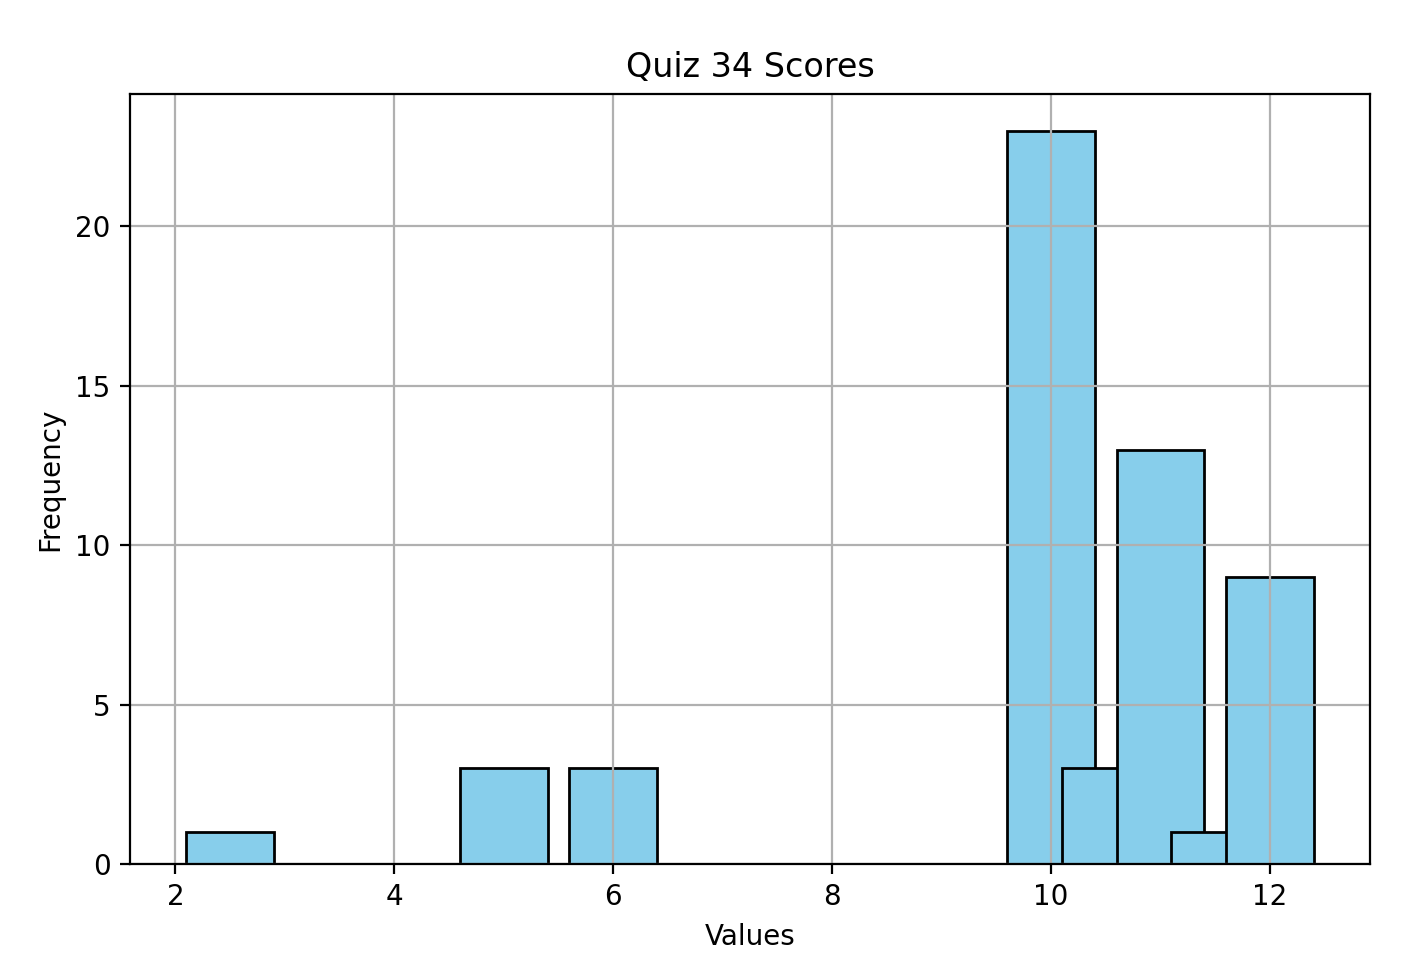
\includegraphics[width=.7\textwidth]{images/reading_quiz_scores}
   		 \caption{Median Score = 10/10 (100\%)}
\end{figure}
\vfill 
\textbf{Grading Rubric.}  	
\begin{enumerate}
\item 10 point for question on expectations.
\item 2 points extra credit for question on variance.
\end{enumerate}

\end{frame}	


\begin{frame}[standout]
Today's quiz
\end{frame}

\begin{frame}
\begin{myredbox}[title=Reading Quiz (Recurrence Relations)]
Solve the recurrence relation $a_n = 5 a_{n-1} + 3$ with initial condition $a_0=1$.
\end{myredbox}
\vfill 

A proposition which may be useful for the reading quiz is given below.

\vfill

\begin{mygreenbox}[title=\text{Proposition 23.1 from Scheinerman}]
All solutions to the recurrence relation $a_n = s a_{n-1} + t$ where $s \neq 1$ have the form
\[a_n = c_1 s^n + c_2, \]
where $c_1$ and $c_2$ are specific numbers.
\end{mygreenbox} 

\end{frame}



\begin{frame}[standout]
Thoughts on Recurrence
\end{frame}

\begin{frame}{Three ways to define sequences}

\colorbox{green!30}{\textbf{1. Writing the first few terms.}} E.g.: Consider the sequence $3,5,7,\hdots.$ \pause 
\vfill 
\colorbox{red!30}{\textbf{Problem.}} \pause   \underline{Misunderstandings} can occur.  \pause The next sequence could be 9 (if we mean odd integers) or 11 (if we mean odd prime integers). \pause 
\vfill\vfill 
\colorbox{green!30}{\textbf{2. State a recurrence relation.}} \pause E.g. $a_n = 5 a_{n-1} + 3$ with initial condition $a_0=1$. \pause 
\vfill 
\colorbox{red!30}{\textbf{Problem.}} \pause  The \underline{computation} to obtain the $n$-th term can be prohibitive. (See the next few slides.) \pause 
\vfill\vfill 
\colorbox{green!30}{\textbf{3. Give an explicit formula for the $n$-th term.}} E.g.  \pause 
\[ a_n = \frac{7}{4} \cdot 5^n -\frac{3}{4}.\]
\vfill  
\pause \colorbox{yellow!30}{\textbf{Appeal.}} This is the best situation to be in. Clear and quick.  The textbook gives techniques for obtaining these.
\end{frame}


\begin{frame}{Recurrent computer programs are slow}
Consider the program to solve  $a_n = 3 a_{n-1} - 2 a_{n-2}$ with initial conditions $a_0=1, a_1=5$:
    \begin{center}
 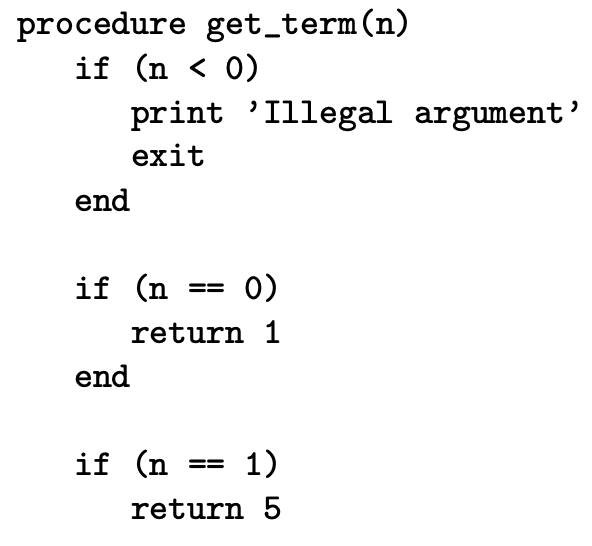
\includegraphics[width=0.475\textwidth]{images/recurrence_program_1} \\ 
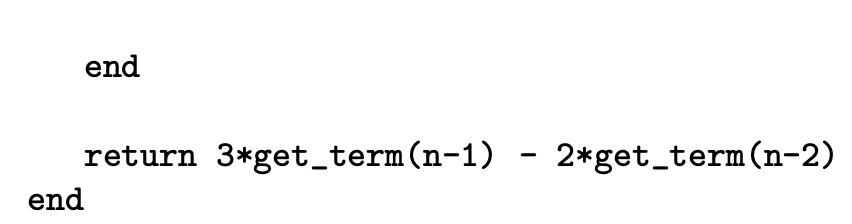
\includegraphics[width=0.475\textwidth]{images/recurrence_program_2} 
     \end{center} 
 \vfill  
\pause \colorbox{yellow!30}{\textbf{Poll.}} How many times is this program called in order to calculate $a_n$?
\end{frame}

\begin{frame}{Recurrent computer programs are slow}

    \begin{center}
 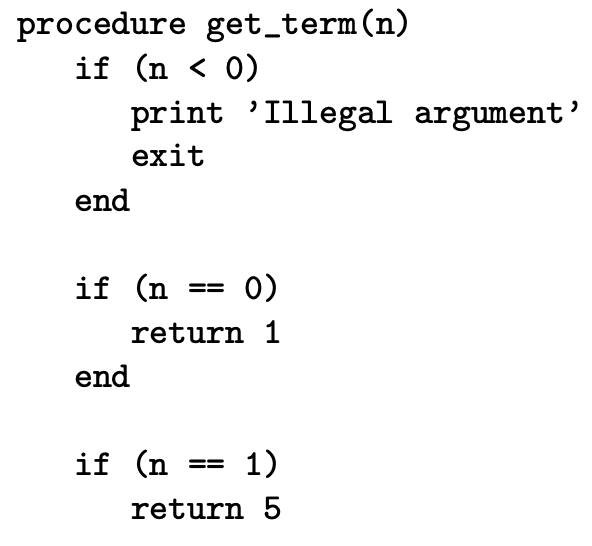
\includegraphics[width=0.4\textwidth]{images/recurrence_program_1} 
    	\vspace{-.1cm} \\
 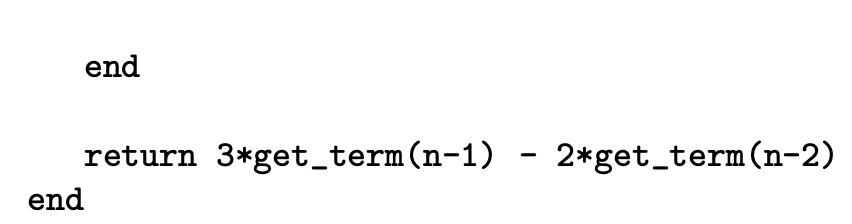
\includegraphics[width=0.4\textwidth]{images/recurrence_program_2} 
     \end{center} 
 \vfill  
%\pause \colorbox{yellow!30}{\textbf{Poll.}} How many times is this program called when it calls $a_n$?
%\vfill 
\colorbox{green!30}{\textbf{Solution.}} 
From the last line, the program is called
\[ b_n = b_{n-1} + b_{n-2} + 1\]
times to get term $a_n$. \\
\vfill \pause 
\colorbox{red!30}{\textbf{Problem.}} This program is expensive to run! To get the 50-th term $a_{50}$, the program must be called $b_{50} \approx 40.7$ billion times!
 
\end{frame}

\begin{frame}{Tower of Hanoi}
In 1883, French mathematician \'{E}douard Lucas invented a puzzle, based on an old Indian legend, called the \textbf{Tower of Hanoi}.

   \begin{center}
 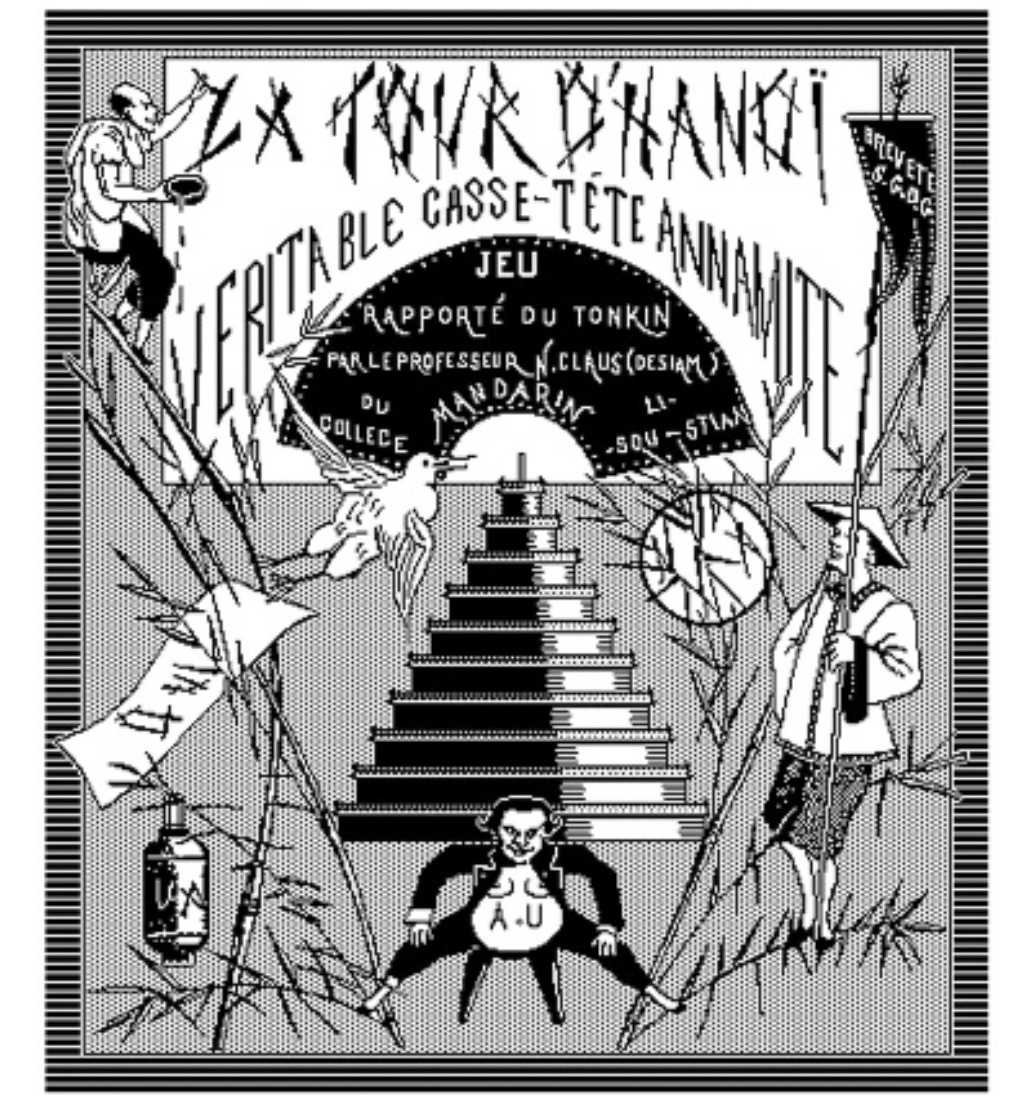
\includegraphics[width=0.4\textwidth]{images/tower_of_hanoi_cover}
   \end{center}

\vfill 
\colorbox{green!30}{\textbf{Prize.}} 
The puzzle offered 10,000 francs (about \$45,000 USD today) to anyone who could solve the puzzle with 64 disks. 

\end{frame}

\begin{frame}{Tower of Hanoi}


   \begin{center}
 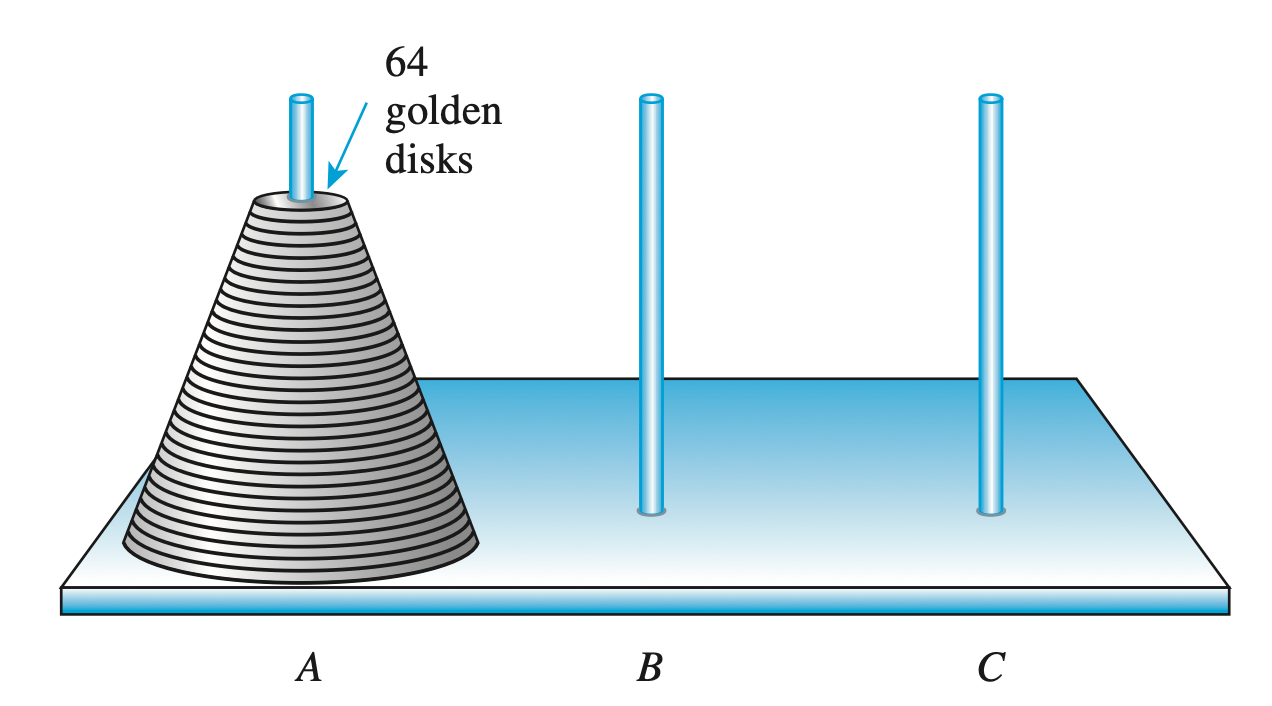
\includegraphics[width=0.7\textwidth]{images/tower_of_hanoi}
   \end{center}

\vfill 
\colorbox{red!30}{\textbf{Rules.}} 
\begin{itemize}
\item You must move all disks one by one from one pole to another.
\item You must never place a larger disk on top of a smaller one.	
\end{itemize}

\end{frame}
	
	
\begin{frame}{Tower of Hanoi: Solution As A Recursion}
    \centering
    \begin{minipage}{0.48\textwidth}
        \centering
        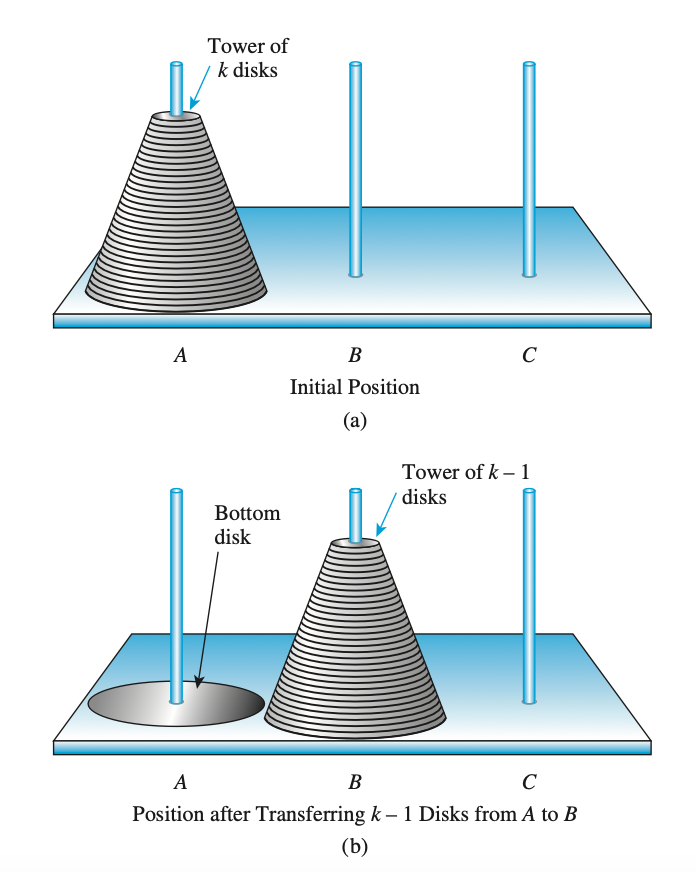
\includegraphics[width=\textwidth]{images/tower_of_hanoi_solution_1}
    \end{minipage}
    \hfill
    \begin{minipage}{0.48\textwidth}
        \centering
     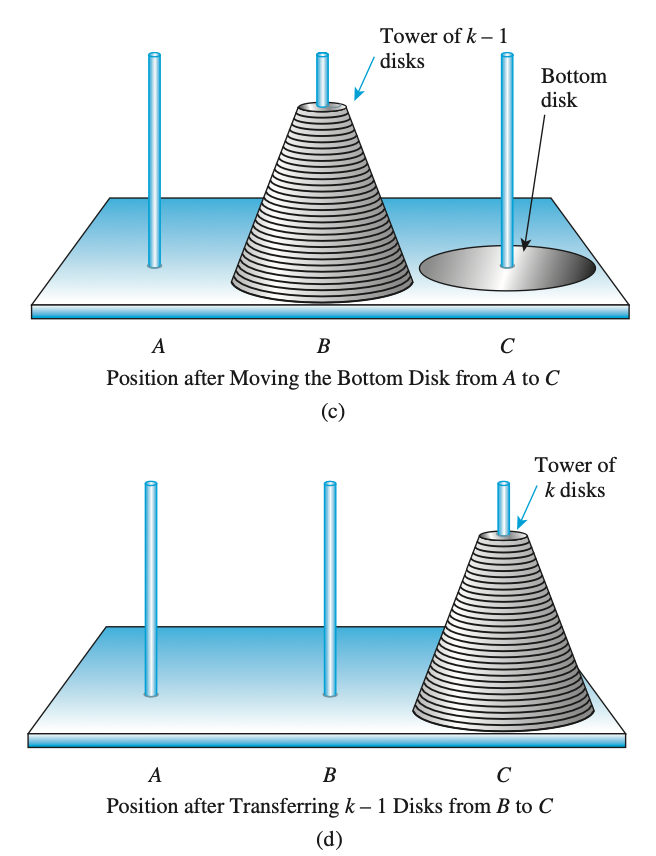
\includegraphics[width=\textwidth]{images/tower_of_hanoi_solution_2}
    \end{minipage}
\end{frame}
	
\begin{frame}{Tower of Hanoi: Solution As A Recursion}

Let $m_k$ be the minimum number of moves needed to transfer a tower of $k$ disks from one pole to another. \\
\vfill 
\colorbox{yellow!30}{\textbf{Poll.}} Can you provide a recursive formula for $m_k$?
\vfill \pause 
\colorbox{green!30}{\textbf{Solution.}} 
From the last slide, we have
%
\begin{align*}
m_k &= m_{k-1} + 1 + m_{k-1} \\
	&= 2 m_{k-1} + 1
\end{align*}
\vfill 
\colorbox{red!30}{\textbf{Remark.}} By solving this recursion, we find  $m_{64} \approx 1.88 \times 10^{19}$.  In other words, if you work rapidly, and move one disk every second, the total number of time it would take to solve the puzzle with 64 disks is: \alert{584.5 billion years}! 
\end{frame}


\begin{frame}{Examples of recursions}

They come up everywhere!  
\vfill 
Some examples from textbooks:

\begin{itemize}
\item Fibonnaci sequence (e.g. for population growth)
\item Compound interest
\end{itemize}
\vfill 
Some examples from real problems:
\begin{itemize}
\item Reinforcement learning	 (e.g. computer chess)
\item Early cancer detection
\end{itemize}
\vfill 
\end{frame}


\begin{frame}[standout]
Group exercises
\end{frame}

\begin{frame}
\footnotesize 
\vfill 
\begin{columns}
\begin{column}{0.33\textwidth}
aaron.loomis: 15 \\ 
adam.wyszynski: 9 \\ 
alexander.goetz: 17 \\ 
alexander.knutson: 1 \\ 
anthony.mann: 19 \\ 
blake.leone: 13 \\ 
bridger.voss: 15 \\ 
caitlin.hermanson: 20 \\ 
cameron.wittrock: 13 \\ 
carsten.brooks: 4 \\ 
carver.wambold: 8 \\ 
colter.huber: 20 \\ 
conner.reed1: 4 \\ 
connor.mizner: 3 \\ 
connor.yetter: 10 \\ 
derek.price4: 18 \\ 
devon.maurer: 11 \\ 
emmeri.grooms: 7 \\ 
erik.moore3: 10 \\ 
ethan.johnson18: 6 \\ 
evan.barth: 9 \\\end{column}
\begin{column}{0.33\textwidth}
evan.schoening: 16 \\ 
griffin.short: 9 \\ 
jack.fry: 14 \\ 
jacob.ketola: 15 \\ 
jacob.ruiz1: 12 \\ 
jacob.shepherd1: 6 \\ 
jada.zorn: 16 \\ 
jakob.kominsky: 21 \\ 
james.brubaker: 2 \\ 
jeremiah.mackey: 14 \\ 
jett.girard: 20 \\ 
john.fotheringham: 16 \\ 
jonas.zeiler: 5 \\ 
joseph.mergenthaler: 17 \\ 
joseph.triem: 5 \\ 
julia.larsen: 3 \\ 
justice.mosso: 13 \\ 
kaden.price: 10 \\ 
lucas.jones6: 8 \\ 
luka.derry: 14 \\ 
luke.donaldson1: 8 \\\end{column}
\begin{column}{0.33\textwidth}
lynsey.read: 12 \\ 
mason.barnocky: 3 \\ 
matthew.nagel: 21 \\ 
micaylyn.parker: 12 \\ 
michael.oswald: 19 \\ 
nolan.scott1: 7 \\ 
owen.obrien: 11 \\ 
pendleton.johnston: 11 \\ 
peter.buckley1: 19 \\ 
reid.pickert: 2 \\ 
ryan.barrett2: 18 \\ 
samuel.hemmen: 1 \\ 
samuel.mosier: 17 \\ 
samuel.rollins: 4 \\ 
sarah.periolat: 7 \\ 
timothy.true: 2 \\ 
tristan.nogacki: 21 \\ 
tyler.broesel: 5 \\ 
william.elder1: 1 \\ 
yebin.wallace: 18 \\ 
zeke.baumann: 6 \\\end{column}
\end{columns}
\vfill
\end{frame}

\begin{frame}{Group exercises}
\begin{enumerate}
	\item Some so-called intelligence tests often include problems in which a series of numbers is presented and the subject is required to find the next term of the sequence.  For example, the sequence might begin 1,2,4,8.  No doubt the examiner is looking for 16 as the next term. \\
	\vspace{.25cm}
	Show how to \enquote{outsmart} the intelligence test by finding a polynomial expression (of degree 3) for $a_n$ such that $a_0=1, a_1=2, a_2=4, a_3=8$, but $a_4=15$.
	\vfill \vfill 
	\item Solve each of the following recurrence relations by giving an explicit formula for $a_n$.  For each, please calculate $a_9$.
	\vspace{.5cm}
	\begin{tabular}{cll}
	\toprule 
	\textbf{Problem} & \textbf{Recurrence relation} & \textbf{Initial condition} \\
	\midrule 
	2a. & $a_n = 3 a_{n-1} -1$ & $ a_0=10$ \\
	2b. &  $a_n = a_{n-1} + 5$ & $  a_0=10$ \\
	2c. & $a_n = 8 a_{n-1} - 15a_{n-2}$ & $a_0=1, \; a_1=4$ \\
	2d. & $a_n = 4 a_{n-1} -4 a_{n-2}$ & $a_0=5, \; a_1=1$ \\
	\bottomrule
	\end{tabular}

\end{enumerate}
\end{frame}


\begin{frame}{Solution to group exercise \#1}
\small 
\textbf{Problem.} [...] Show how to \enquote{outsmart} the intelligence test by finding a polynomial expression (of degree 3) for $a_n$ such that $a_0=1, a_1=2$, $a_2=4, a_3=8$, but $a_4=15$. \\
\vfill 
\textbf{Solution.} We apply Scheinerman Theorem 23.17.
\vspace{-.25cm}
\[
\begin{array}{ccccccccccc}
a:& & 1 &     & 2 &     & 4 &     & 8 &  &15 \\
\Delta a:& &  & 1    &  & 2    &  &  4   &  & 7  & \\
\Delta^2 a:& &  &     & 1 &     & 2 &     &  3 &   & \\
\Delta^3 a:& &  &     &  &  1   & &   1  &   &   & \\
\Delta^4 a:& &  &     &  &     & 0 &     &   &   & \\
\end{array}
\]
Hence $k=3$ and 
%
\begin{align*}
a_n &= a_0 \binom{n}{0} +	\Delta a_0 \binom{n}{1} + 		\Delta^2 a_0 \binom{n}{2} + 		\Delta^3 a_0 \binom{n}{3} \\
&= 1 \binom{n}{0} +	1  \binom{n}{1} + 		1 \binom{n}{2} + 		1 \binom{n}{3} && \scripttext{(Substitute coefs from table)} \\
&= 1 \cdot 1 +	1 \cdot n  + 		1 \cdot \frac{n (n-1)}{2} + 		1 \cdot \frac{n (n-1) (n-2)}{6} && \scripttext{(Expand binomial coefs.)} \\
&= \frac{1}{6} n^3 + \frac{5n}{6} + 1 && \scripttext{(Algebra)}
\end{align*}


\end{frame}


\begin{frame}{Solution to group exercise \#2: Overview}
\footnotesize 
Group exercise \#2 asks us to deduce explicit formulas for $a_n$ from recurrence relations.  

\vfill 

\colorbox{green!30}{\textbf{First Order Recurrence.}} A first order recurrence takes the form
\[ a_n = s a_{n-1}+ t\]
The explicit solution depends on the context 
\[
\begin{array}{cccccc}
\textbf{Context} && \textbf{Solution} && \textbf{Justification} \\
\text{If } s \neq 1 & & a_n = c_1 s^n + c_2 && \text{Prop 23.1} \\
\text{If } s =1 & & a_n = a_0 + nt && \text{Prop 23.3} 
\end{array}
\]

\vfill 

\colorbox{green!30}{\textbf{Second Order Recurrence.}}  A second order recurrence takes the form
\[ a_n = s_1 a_{n-1} + s_2 a_{n-2} \]
The explicit solution depends on the context. First, we solve the quadratic formula $x^2 - s_1 x - s_2 =0$ to find roots $r_1$ and $r_2$.
\[
\begin{array}{cccccc}
\textbf{Context} && \textbf{Solution} && \textbf{Justification} \\
\text{If } r_1 \neq r_2  & & a_n = c_1 r_1^n + c_2 r_2^n && \text{Thm 23.5} \\
\text{If } r_1 = r_2 \defeq r & & a_n = c_1 r^n + c_2 n r^n && \text{Thm 23.9} 
\end{array}
\]

\vfill 

\colorbox{red!30}{\textbf{Remark.}} Whenever the solution involves unknown constants (denoted $c_1$ and $c_2$), you must solve for them. You do this by plugging in the first two values for the sequence ($a_0$ and $a_1$) along with other known values (some subset of $\set{s^n, t, r_1^n, r_2^n, r^n, nr^n}$) to form a system of two equations with two unknowns.  Then solve the system (e.g. using substitution).   

\end{frame}

\begin{frame}{Solution to group exercise \#2a}

\textbf{Problem.} Solve the recurrence relation $a_n = 3 a_{n-1} -1$ with initial condition $a_0=10$ to give an explicit formula for $a_n$. 

\vfill 
	
\textbf{Solution.} By Prop 23.1, the solution takes the form 
%
\begin{align*}
a_n &= c_1 s^n + c_2 \\
\implies a_n &= c_1 \cdot 3^n + c_2
\end{align*}
%
Substituting in the provided initial condition $a_0=10$ and the next term of the sequence $a_1 =29$, we obtain the system of equations
%
\begin{align*}
10 &= c_1 + c_2 \\
29 &= 3c_1 + c_2
\end{align*}
%
Solving this system yields $c_1 = 9.5$ and $c_2 = 0.5$.  Hence, the final solution is
\[ a_n = 9.5 \cdot 3^n + 0.5 \]


\end{frame}


\begin{frame}{Solution to group exercise \#2b}

\textbf{Problem.} Solve the recurrence relation  $a_n = a_{n-1} + 5$  with initial condition $a_0=10$ to give an explicit formula for $a_n$. 

\vfill 
	
\textbf{Solution.} By Prop 23.2, the solution takes the form 
%
\begin{align*}
a_n = a_0 + nt
\end{align*}
%
Substituting in the provided initial condition $a_0=10$ and the given $t=5$, we obtain the final solution 
\[ a_n = 10 + 5n \]

\end{frame}

\begin{frame}{Solution to group exercise \#2c}
\footnotesize
\textbf{Problem.} Solve the recurrence relation $a_n = 8 a_{n-1} - 15a_{n-2}$  with initial conditions $a_0=1$ and $a_1=4$ to give an explicit formula for $a_n$. 
\vfill  \vfill 
\textbf{Solution.} First, we solve the quadratic formula 
%
\begin{align*}
& x^2 - s_1 x - s_2 =0  \\
\implies & x^2 - 8 x + 15 =0  \\
\implies & (x-5)(x-3) =0  
\end{align*}
%
Hence the roots are $r_1=5$ and $r_2=3$.  Since these roots are distinct, we apply Thm 23.5, which tell us that the solution takes the form 
%
\begin{align*}
a_n &= c_1 r_1^n + c_2 r_2^n \\
\implies a_n &= c_1 5^n + c_2 3^n 
\end{align*}
%
Substituting in the provided initial conditions  $a_0=1$ and $a_1=4$, we obtain the system of equations
%
\begin{align*}
1 &= c_1 + c_2 \\
4 &= 5c_1 + 3c_2
\end{align*}
%
Solving this system yields $c_1 = \half$ and $c_2 = \half$.  Hence, the final solution is
\[ a_n = \half \cdot  5^n + \half \cdot 3^n  \]


\end{frame}

\begin{frame}{Solution to group exercise \#2d}
\footnotesize
\textbf{Problem.} Solve the recurrence relation $a_n = 4 a_{n-1} -4 a_{n-2}$  with initial conditions $a_0=5$ and $a_1=1$ to give an explicit formula for $a_n$. 
\vfill  \vfill 
\textbf{Solution.} First, we solve the quadratic formula 
%
\begin{align*}
& x^2 - s_1 x - s_2 =0  \\
\implies & x^2 - 4 x + 4 =0  \\
\implies & (x-2)(x-2) =0  
\end{align*}
%
Hence the roots are $r_1=2$ and $r_2=2$.  Since these roots are identical, we apply Thm 23.9, which tell us that the solution takes the form 
%
\begin{align*}
a_n &= c_1 r^n + c_2 n r^n \\
\implies a_n &= c_1 2^n + c_2 n 2^n 
\end{align*}
%
Substituting in the provided initial conditions  $a_0=5$ and $a_1=1$, we obtain the equations
%
\begin{align*}
5 &= c_1  \\
1 &= 2c_1 + 2c_2
\end{align*}
%
Solving these equations yields $c_1 = 5$ and $c_2 = -4.5$.  Hence, the final solution is
\[ a_n = 5 \cdot  2^n -4.5 \cdot n 2^n  \]


\end{frame}


\end{document}
